%%%%%%%%%%%%%%%%%%%%%%%%%%%%%%%%%%%%%%%%%%%%%%%%%%%%%%%%%%%%%%%%%%%%
%% I, the copyright holder of this work, release this work into the
%% public domain. This applies worldwide. In some countries this may
%% not be legally possible; if so: I grant anyone the right to use
%% this work for any purpose, without any conditions, unless such
%% conditions are required by law.
%%%%%%%%%%%%%%%%%%%%%%%%%%%%%%%%%%%%%%%%%%%%%%%%%%%%%%%%%%%%%%%%%%%%

%\documentclass[notes]{beamer}       % print frame + notes
%\documentclass[notes=only]{beamer}   % only notes
\documentclass{beamer} 
\usetheme[faculty=phil]{fibeamer}
\usepackage[utf8]{inputenc}
\usepackage[
  main=english, %% By using `czech` or `slovak` as the main locale
                %% instead of `english`, you can typeset the
                %% presentation in either Czech or Slovak,
                %% respectively.
]{babel}        %% typeset as follows:
%%
%%   \begin{otherlanguage}{czech}   ... \end{otherlanguage}
%%   \begin{otherlanguage}{slovak}  ... \end{otherlanguage}
%%
%% These macros specify information about the presentation
% TODO: The date
\title{Examination Timetabling Problem} %% that will be typeset on the
\subtitle{Optimization Methods and Algorithms\\Group 9} %% title page.
\author{s252894 - Piero Macaluso\\s246422 - Ludovico Pavesi\\s254036 - Alberto Romano\\s217189 - Lorenzo Manicone\\s246422 - Donato Tortoriello}
%% These additional packages are used within the document:
\usepackage[]{algorithm2e}

\usepackage{ragged2e}  % `\justifying` text
\usepackage{booktabs}  % Tables
\usepackage{tabularx}
\usepackage{tikz}      % Diagrams
\usetikzlibrary{calc, shapes, backgrounds}
\usepackage{amsmath, amssymb}
\usepackage{url}       % `\url`s
\usepackage{listings}  % Code listings
\frenchspacing
\hypersetup{pdfpagemode=FullScreen}
\begin{document}
  \frame{\maketitle
 		\note{\textbf{Piero}: Hi, we are the Group 9 of the course Optimization Methods and Algorthms. This group is composed by me, Piero Macaluso, Ludovico Pavesi, Alberto Romano, Lorenzo Manicone and Donato Tortoriello.}}
	\begin{frame}<beamer>
	\frametitle{Outline}
	\tableofcontents
\end{frame}
  \AtBeginSection[]{% Print an outline at the beginning of sections
    \begin{frame}<beamer>
      \frametitle{Outline}
      \tableofcontents[currentsection]
    \end{frame}}
	
	\section{Introduction}
	\begin{frame}
	\note{\textbf{Ludovico}: In our code we decided to use Simulated Annealing Metaheuristic with an implementation of Local Search and Timeslot swap. We managed to implement our code using thread in order to give to create n different path of research at the same time. The only thing that is in common and represents the critical part is the current best. Only one thread can access to the best cost at the same time.}
	\frametitle{\thesection \ \insertsection}
	Our algorithm is based on:
	\begin{itemize}
		\item Simulated annealing with mutations
		\item Local search
		\item Swapping time slots
		\item Multistart
	\end{itemize}
	\end{frame}
	
   \section{Initial solution generation}
   
   \subsection{Scheduling Exams}

	\begin{frame}
	   \frametitle{\thesection.\thesubsection \ \insertsubsection}
	   \framesubtitle{Ordering Exams}
	   
	\textbf{Goal}: \alert{sort} in a useful way the whole set of exams:
	\begin{block}{Number of Unavailable Time Slots}
		The number of time slots where there are exams in conflict with current one.
	\end{block}
	\begin{block}{Number of Conflicts}
		The (constant) number of conflicting exams with current one.
	\end{block}
	\end{frame}

\begin{frame}
\frametitle{\thesection.\thesubsection \ \insertsubsection}
\framesubtitle{The First Critical Point}
\begin{alertblock}{No More Available Time Slots}
	In most instances our program got stuck because when almost all exams have been scheduled, remaining ones have no available time slots.
\end{alertblock}
%\pause
\begin{block}{Solution}
	 If the algorithm detects that it got stuck, it tries to ``escape'' by \alert{unscheduling all conflicting exams} and continuing to loop until all exams have been scheduled.
\end{block}

\end{frame}

\begin{frame}
\frametitle{\thesection.\thesubsection \ \insertsubsection}
\framesubtitle{The Second Critical Point}
\begin{alertblock}{Unstable situations}
	Sometimes the algorithm loops for too long or forever: it keeps unscheduling exams and never manages to schedule all of them.

\end{alertblock}
%\pause
\begin{block}{Solution}
	Setting a maximum number of retries (``unschedule all conflicting exams''). If limit is reached, return an incomplete solution that will be discarded. % il fatto che viene chiamato in un while e quindi riprova alla slide dopo
\end{block}

\end{frame}

	\begin{frame}
	\frametitle{\thesection.\thesubsection \ \insertsubsection}
	\framesubtitle{The Pseudo-Code}
	\begin{columns}[onlytextwidth]
	\column{.65\textwidth}
	\scalebox{.6}{
	\begin{algorithm}[H]
		%		$backup \gets \text{current solution (even an empty one)}$\;
		%		$sol \gets \text{current solution (even an empty one)}$\;
		$retries \gets 0$\;
		$list \gets \text{exams to be scheduled}$\;
		sort $list$\;
		\While{$list$ is not empty}{
			\If{\textit{retries} > limit}{
				\Return{\alert{no feasible solution found}}\;
				%				$sol \gets backup$\;
				%				restart the alogithm\;
			}
			$E \gets \textit{ first element from }list$\;
			$T \gets \textit{ random available time slot}$\;
			\eIf{$T$ is valid (not null)}{
				schedule $E$ in $T$\;
				remove $E$ from $list$\;
			}{
				\ForEach{conflicting exam $C$ of $E$}{
					unschedule $C$\;
				}
				$retries \gets retries + 1$\;
			}
			sort $list$ again\;
		}
		\Return{\alert{feasible solution found}}\;
	\end{algorithm}}
	\column{.35\textwidth}
\begin{block}{While Loop}
	This code is in a while loop that continues to loop till the code returns \textbf{true}.
\end{block}
\end{columns}
	\end{frame}

	

   \subsection{Local Search}
   
   \begin{frame}
   \frametitle{\thesection.\thesubsection \ \insertsubsection}
   \framesubtitle{Characteristics of Local Search}
   	
   \begin{itemize}
   	\item Try to place every exam in currently best available time slot
   	\item Best Improvement
   	\item Generation of Neighborhood: O($e$)
   	\item Solution Evaluation: O($e$)
   	\item Real case less than O($e^2$), on average
   	\item Repeats while improvement is above a minimum threshold
   \end{itemize}
 
\end{frame}

	\begin{frame}
	   \frametitle{\thesection.\thesubsection \ \insertsubsection}
	   \framesubtitle{The Pseudo-Code}
	   	\begin{columns}[onlytextwidth]
	   		\column{1\textwidth}
	   \scalebox{.7}{
	\begin{algorithm}[H]
		%		$sol \gets \text{current solution (even an empty one)}$\;
		$list \gets \text{all exams to be scheduled, sorted by }\textit{number of conflicts}$\;
		\ForEach{exam $E$ in $list$}{
			$T \gets \text{time slot where }E\text{ is scheduled}$\;
			$C \gets \text{cost of }E\text{ in }T\text{ according to objective function}$\;
			\ForEach{time slot $T'\neq T$}{
				$C' \gets \text{cost of }E\text{ in }T'\text{ according to objective function}$\;
				\If{$C'<C$}{
					schedule $E$ in $T'$\;
					$C \gets C'$\;
				}
			}
		}
	\end{algorithm}}
\end{columns}
	\end{frame}

\begin{frame}
\frametitle{\thesection.\thesubsection \ \insertsubsection}
\framesubtitle{Results}

\begin{itemize}
	\item Provides the initial delta for Simulated Annealing
	\item Minimum improvement of 10\% works well with given instances (1-2 iterations)
	\item Stops in around 5 iterations even with 0.001\%
	\item Minimum improvement depends on temperature % magari si può dire per spiegare il punto di sopra, o vice versa, per non scrivere proprio TUTTO?
\end{itemize}

\end{frame}

\section{Simulated Mutant Annealing}

\subsection{Parameter Calibration}

\begin{frame}
\frametitle{\thesection.\thesubsection \ \insertsubsection}
\framesubtitle{Initial Temperature}
	According to the theory of Simulated Annealing, the probability $p$ of taking a worse solution is described by:
	\begin{gather}\label{eq:3.1}
	p = e^{\frac{-(F(x)-F(\tilde{x}))}{T}}\\
\begin{aligned}
\text{where } &F(x) \text{ is the solution cost of the current solution}\\
&F(\tilde{x}) \text{ is the solution cost of the neighbor}\\
&T \text{ is the current temperature}
\end{aligned}\notag
	\end{gather}
	
\vfill
\begin{itemize}
	\item The lower is the temperature, the lower is the probability
	\item The higher is the delta, the lower is the probability
\end{itemize}

\end{frame}
\begin{frame}
\frametitle{\thesection.\thesubsection \ \insertsubsection}
\framesubtitle{Initial Temperature}
\begin{itemize}
	\item Starting Probability 0.5
	\item $F(\tilde{x})-F(x)$ is the initial delta ($\Delta$)
\end{itemize}
\begin{gather}\label{eq:3.2}
0.5 = e^{\frac{\Delta}{T}}\notag\\
log(0.5) = \frac{\Delta}{T}\notag\\
T = \frac{\Delta}{log(0.5)}\\\notag
\end{gather}

\begin{itemize}
	\item Different temperature for different instances
\end{itemize}

\end{frame}

\subsection{Neighbor Generation/Mutation}

\begin{frame}
\frametitle{\thesection.\thesubsection \ \insertsubsection}
\framesubtitle{Mutant Neighbor}
\begin{enumerate}
	% TODO: abbozzo
	\item Generate a neighbor by \alert{unscheduling a percentage of exams} and rescheduling them
	\item Apply local search
	\item Apply time slot swapping
	\item Compare with current (thread-local) solution
	\item If improved, also compare with global best
\end{enumerate}
\end{frame}

\begin{frame}
\frametitle{\thesection.\thesubsection \ \insertsubsection}
\framesubtitle{Parameter tuning}
\begin{itemize}
	% TODO: abbozzo
	\item Percentages decrease with temperature % non "linearly" perché unscheduled si ferma a 10% anche se andrebbe sotto, non è lineare
	\item Unscheduled exams from 30\% to 10\%
	\begin{itemize}
		\item More than 50\% too slow, 10\% mixed results % "below 10% was pointless" si aggiunge a voce
	\end{itemize}
	\item Local search minimum improvement from 10\% to almost 0\%
\end{itemize}
\end{frame}

\subsection{Time Slot Swap}

\begin{frame}
\frametitle{\thesection.\thesubsection \ \insertsubsection}
\
\begin{itemize}
	% TODO: abbozzo
	\item Try to swap every couple of time slots % sorvoliamo sulla complessità
	\item Big improvements on most instances
	\item Local search, then swap
	\item Other way around didn't work very well on instance 6
\end{itemize}
\end{frame}

\section{Conclusions}

\subsection{Statistics}

\begin{frame}
\frametitle{\thesection.\thesubsection \ \insertsubsection}
\framesubtitle{CandleStick Chart of Gaps}
	\scalebox{0.4}{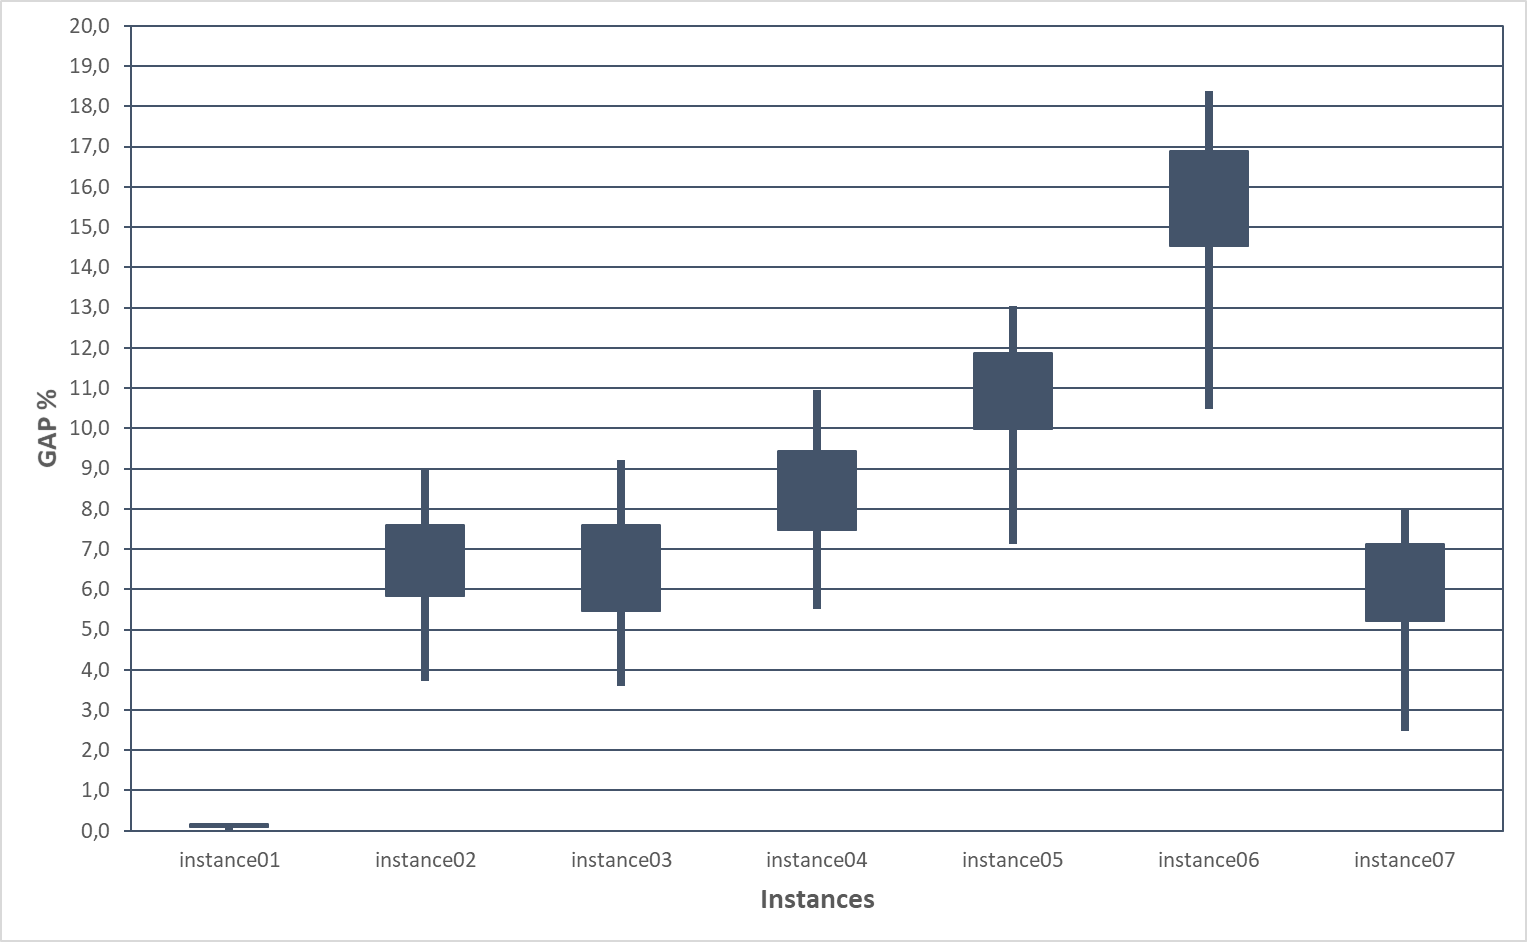
\includegraphics{resources/candlelight.png}}
\end{frame}

\begin{frame}
\frametitle{\thesection.\thesubsection \ \insertsubsection}
\framesubtitle{Some Considerations}
\begin{itemize}
	% TODO: abbozzo
	\item \textit{Instance01} is the \alert{best}, \textit{Instance06} is the \alert{worst}
	\item Average gap around 8\% elsewhere
	\item Standard deviation relatively small and constant across instances
	\item Denser instances like 2 and 7 sometimes give ``exceptional'' results (lower minimum)
	\item Benchmarking script
\end{itemize}
\end{frame}

\subsection{Source Code}

\begin{frame}
\frametitle{\thesection.\thesubsection \ \insertsubsection}
\framesubtitle{See more on Github}
Thanks for listening.
\vfill
Our source code is avalable on Github: \href{https://github.com/pimack/OMA9}{\underline{github.com/pimack/OMA9}}
\end{frame}

\end{document}
po